\documentclass[12pt]{article}
\usepackage{amsmath, amsfonts, amssymb}
\usepackage{graphicx}
\DeclareMathOperator*{\argmax}{arg\,max}
\DeclareMathOperator*{\argmin}{arg\,min}
\DeclareMathOperator{\diag}{diag}
\DeclareMathOperator{\rank}{rank}
\title{Least-Squares Estimation}
\author{J\'{e}r\^{o}me Maye}
\date{\today}
\begin{document}
  \maketitle

  \section{1D Case}
    Let us define a set of $n$ realizations $\{y_i\}_{i=1}^n\in\mathbb{R}$ of an
    observable random variable $Y$ such that

    \begin{equation}\label{eqn:model1d}
      \begin{aligned}
        Y \sim p(f(X),\boldsymbol{\Theta}),
      \end{aligned}
    \end{equation}

    \noindent where $X\in\mathbb{R}^d$ is a latent random variable, $f(\cdot)$
    an arbitrary function of $\mathbf{X}$, $p(\cdot)$ a probability density
    function, and $\boldsymbol{\Theta}$ its known parameters. In other words, we
    can state that

    \begin{equation}\label{eqn:model1dreal}
      \begin{aligned}
        \epsilon_i \sim p(\boldsymbol{\Theta}), i = 1\cdots n\\
        y_i = f(x_i) + \epsilon_i, i=1\cdots n,
      \end{aligned}
    \end{equation}

    \noindent where $\{x_i\}_{i=1}^n$ are realizations of $\mathbf{X}$.

    We can define the \emph{residuals} as

    \begin{equation}\label{eqn:model1dres}
      \begin{aligned}
      e_i = y_i - f(x_i),
      \end{aligned}
    \end{equation}

    \noindent which are distributed according to

    \begin{equation}\label{eqn:model1dresdist}
      \begin{aligned}
      E \sim p(\boldsymbol{\Theta}),
      \end{aligned}
    \end{equation}

    \noindent where $E$ is a random variable whose realizations are $e_i$.

    In order to estimate $\mathbf{X}$, one can use Maximum Likelihood Estimation
    (MLE) and derive the likelihood of the residuals

    \begin{equation}\label{eqn:model1dlikelihood}
      \begin{aligned}
      p(e_{1\cdots n}\mid\mathbf{X},\boldsymbol{\Theta}) =
        \prod_i^n p(e_i\mid\mathbf{X},\boldsymbol{\Theta}).
      \end{aligned}
    \end{equation}

    The likelihood function is

    \begin{equation}\label{eqn:model1dlikelihoodfunction}
      \begin{aligned}
      \mathcal{L}(\mathbf{X}) = p(e_{1\cdots n};\mathbf{X},\boldsymbol{\Theta}) =
        \prod_i^n p(e_i;\mathbf{X},\boldsymbol{\Theta}).
      \end{aligned}
    \end{equation}


    The sought estimate for $\mathbf{X}$ is then found by maximizing
    \eqref{eqn:model1dlikelihoodfunction}

    \begin{equation}\label{eqn:model1dmaxl}
      \begin{aligned}
      \mathbf{\hat{X}} = \argmax_{\mathbf{X}}\mathcal{L}(\mathbf{X}),
      \end{aligned}
    \end{equation}

    which is turned into

    \begin{equation}\label{eqn:model1dminll}
      \begin{aligned}
      \mathbf{\hat{X}} =
      \argmin_{\mathbf{X}}\sum_i^n -\ln(p(e_i;\mathbf{X},\boldsymbol{\Theta})).
      \end{aligned}
    \end{equation}

    \subsection{Normally Distributed Residuals with Equal Variances}

      Let us consider the case

      \begin{equation}\label{eqn:model1dnormresidualssim}
        \begin{aligned}
        e_i \sim \mathcal{N}(0, \sigma^2),
        \end{aligned}
      \end{equation}

      \noindent where $\sigma^2$ is the variance of the residuals and therefore

      \begin{equation}\label{eqn:model1dnormresidualspdf}
        \begin{aligned}
        p(e_i\mid\mathbf{X},\boldsymbol{\Theta}) = \frac{1}{\sqrt{2\pi\sigma^2}}
          \exp(-\frac{e_i^2}{2\sigma^2}).
        \end{aligned}
      \end{equation}

      Therefore, \eqref{eqn:model1dminll} becomes

      \begin{equation}\label{eqn:model1dminllnorm}
        \begin{aligned}
        \mathbf{\hat{X}} &=
          \argmin_{\mathbf{X}}\frac{n}{2}\ln(2\pi\sigma^2) +
          \frac{1}{2\sigma^2}\sum_i^n e_i^2 \\&=
        \argmin_{\mathbf{X}}\sum_i^n e_i^2 \\&=
        \argmin_{\mathbf{X}}\sum_i^n (y_i-f(x_i))^2,
        \end{aligned}
      \end{equation}

      \noindent which is the standard formulation of a \emph{least-squares}
      problem.

    \subsection{Normally Distributed Residuals with Unequal Variances}

      Let us consider the case

      \begin{equation}\label{eqn:model1dnormresidualssim2}
        \begin{aligned}
        e_i \sim \mathcal{N}(0, \sigma_i^2),
        \end{aligned}
      \end{equation}

      \noindent where $\sigma_i^2$ is the variance of residual $e_i$.

      In that case, the formulation becomes

      \begin{equation}\label{eqn:model1dminllnorm2}
        \begin{aligned}
        \mathbf{\hat{X}} &=
          \argmin_{\mathbf{X}}\sum_i^n \frac{1}{\sigma_i^2}(y_i-f(x_i))^2,
        \end{aligned}
      \end{equation}

      \noindent which corresponds to a \emph{weighted least-squares} problem.

    \subsection{Normally Distributed Residuals with Outliers}

      For this problem, we can define residual distributions that have heavier
      tails. The outliers will thus be more likely than with the normal
      distribution.

      A typical method for these kind of problems are \emph{M-Estimators}. The
      least-squares problem is formulated as

      \begin{equation}\label{eqn:model1dMEstimator}
        \begin{aligned}
        \mathbf{\hat{X}} &=
          \argmin_{\mathbf{X}}\sum_i^n w(e_i)e_i^2,
        \end{aligned}
      \end{equation}

      \noindent where $w(e_i)$ is a weight function. In the trivial case where
      we consider normally distributed residuals, the weight function is
      not dependent on the value of $e_i$, i.e., $w(e_i)=\frac{1}{\sigma^2}$ or
      $w(e_i)=\frac{1}{\sigma_i^2}$ in case of unequal variances. In the other
      cases, it can be considered as an
      \emph{iteratively reweighted least-squares} problem.

      \subsubsection{Modified Blake-Zisserman M-Estimator}

        The modified Blake-Zisserman M-Estimator defines

        \begin{equation}\label{eqn:model1dnormresidualspdfbz}
          \begin{aligned}
          p(e_i\mid\mathbf{X},\boldsymbol{\Theta}) =
            \frac{1}{\sqrt{2\pi\sigma^2}}
            \exp(-\frac{e_i^2}{2\sigma^2}) + \varepsilon,
          \end{aligned}
        \end{equation}

        \noindent where $\varepsilon$ is a parameter. Note that
        \eqref{eqn:model1dnormresidualspdfbz} is not a proper probability
        density function. The cost function associated with
        \eqref{eqn:model1dnormresidualspdfbz} approximates the standard
        least-squares cost function for inliers while it asymptotically tends
        to $-\log(\varepsilon)$ for outliers.

        The weight function is defined as

        \begin{equation}\label{eqn:model1dwbz}
          \begin{aligned}
          w(e_i) = \frac{\frac{1}{\sqrt{2\pi\sigma^2}}
            \exp(-\frac{e_i^2}{2\sigma^2})}
            {(\frac{1}{\sqrt{2\pi\sigma^2}}\exp(-\frac{e_i^2}{2\sigma^2}) +
            \varepsilon)\sigma^2}.
          \end{aligned}
        \end{equation}

        We can analyze the behavior of this estimator on a simple example.
        $1000$ residuals are generated according to
        $e_i\sim\mathcal{N}(0,1e^{-3})$. Fig.~\ref{fig:bz1} shows the residuals
        and their respective weights for different values of $\varepsilon$.
        As $\varepsilon$ tends to zero, the weights become constant and thus
        this corresponds to the standard least-squares problem.

        \begin{figure}[t]
          \centering
          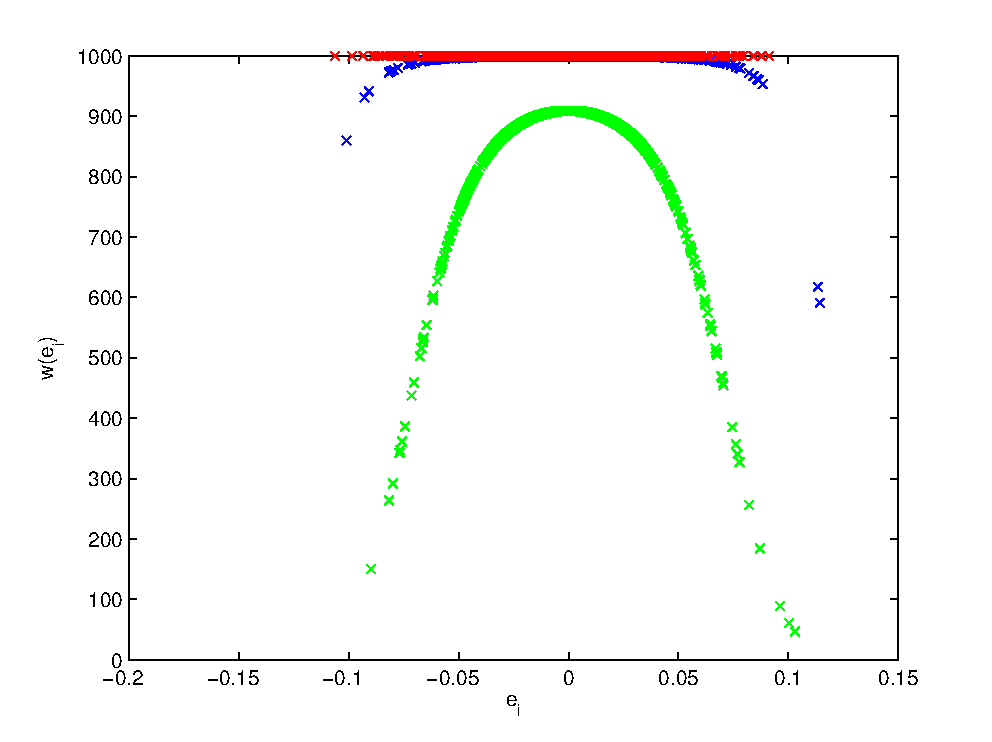
\includegraphics[scale=0.7]{bz.pdf}
          \caption{Normally distributed residuals and their weights with
            different values of
            $\varepsilon$. The red crosses corresponds to $\varepsilon=1e^{-6}$,
            the blue to $\varepsilon=1e^{-3}$, and the green to
            $\varepsilon=1e^{-1}$.}
          \label{fig:bz1}
        \end{figure}

        The introduction of outliers leads to a more interesting problem. Let
        us now generate $900$ residuals according to
        $e_i\sim\mathcal{N}(0,1e^{-3})$ and $100$ according to
        $e_i\sim\mathcal{N}(\mathcal{U}(-100,100),1e^{-3})$. Fig.~\ref{fig:bz2}
        shows the residuals and their weights. The outliers receive a weight
        close to zero and therefore do not perturbate the cost function.

        \begin{figure}[t]
          \centering
          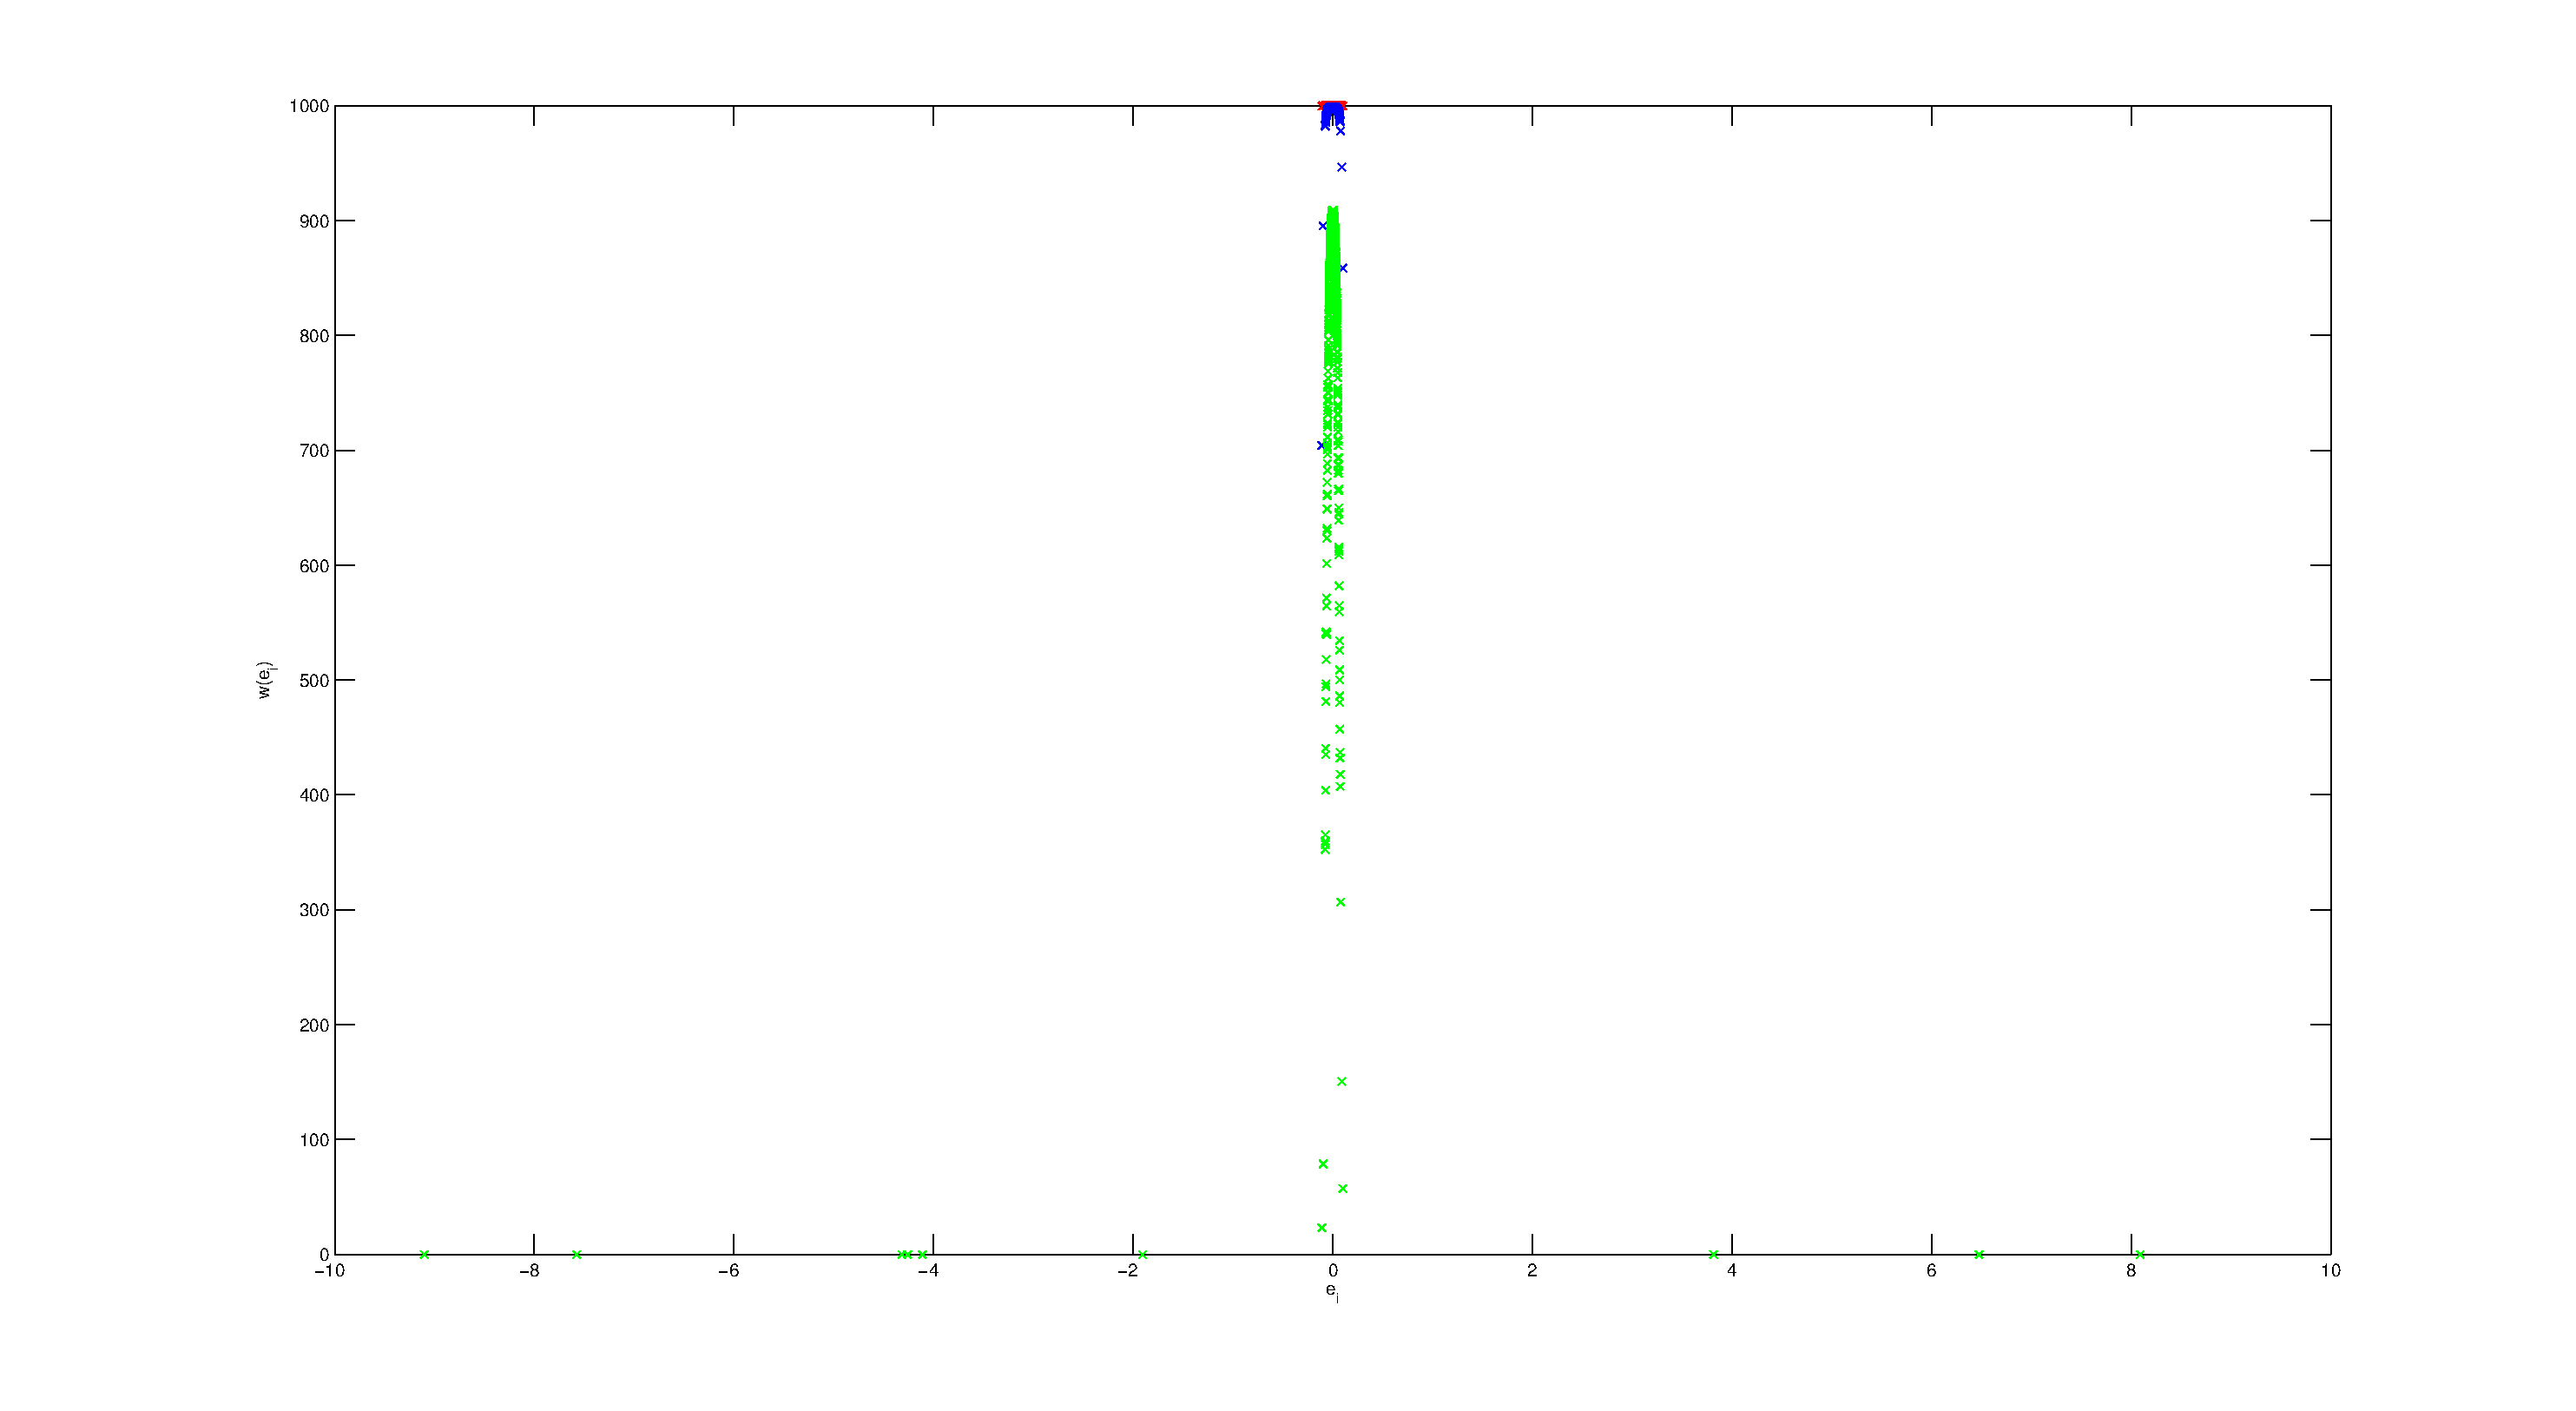
\includegraphics[scale=0.3]{bz2.pdf}
          \caption{Normally distributed residuals with outliers and their
            weights with
            different values of
            $\varepsilon$. The red crosses corresponds to $\varepsilon=1e^{-6}$,
            the blue to $\varepsilon=1e^{-3}$, and the green to
            $\varepsilon=1e^{-1}$.}
          \label{fig:bz2}
        \end{figure}

        From statistical theory, we know that approximately $99.7\%$ of the
        samples of a zero-centered normal distribution lie within the interval
        $[-3\sigma,3\sigma]$. Therefore, we would like to tailor $\varepsilon$
        such that these samples receive a similar weight as with the standard
        least-squares cost function.

\end{document}
